%Dokumentation: http://texdoc.net/
\documentclass[a4paper,twocolumn,twoside]{article}
\usepackage[a4paper]{geometry}

\usepackage[british]{babel}        
\usepackage[utf8]{inputenc}        % for umlauts and other non 7bit ascii things
\usepackage[T1]{fontenc}           % this is needed for correct output of umlauts in pdf
\usepackage{lmodern}               % use a vector based font, not a bitmap based font for T1
\usepackage[stretch=10]{microtype} % improves font placements
%\usepackage{graphicx}
\usepackage[breaklinks, colorlinks,draft=false
, citecolor=black, filecolor=black, linkcolor=black, urlcolor=black ,pdfborder=0
]{hyperref}


\usepackage{listings}
\usepackage{color}

\definecolor{codegreen}{rgb}{0,0.6,0}
\definecolor{codegray}{rgb}{0.5,0.5,0.5}
\definecolor{codepurple}{rgb}{0.58,0,0.82}
\definecolor{backcolour}{rgb}{0.95,0.95,0.92}

\lstdefinestyle{pseudostyle}{
	backgroundcolor=\color{backcolour},   
	commentstyle=\color{codegreen},
	keywordstyle=\color{magenta},
	numberstyle=\tiny\color{codegray},
	stringstyle=\color{codepurple},
	basicstyle=\footnotesize,
	breakatwhitespace=false,         
	breaklines=true,                 
	captionpos=b,                    
	keepspaces=true,                 
	numbers=left,                    
	numbersep=5pt,                  
	showspaces=false,                
	showstringspaces=false,
	showtabs=false,                  
	tabsize=2
}

% Define Language
\lstdefinelanguage{Pseudo}
{
	% list of keywords
	morekeywords={
		Click
	},
	sensitive=false, % keywords are not case-sensitive
	morecomment=[l]{//}, % l is for line comment
	morecomment=[s]{/*}{*/}, % s is for start and end delimiter
	morestring=[b]" % defines that strings are enclosed in double quotes
}


\usepackage{mathtools}
\usepackage{amsfonts}
\usepackage{amsthm}
\usepackage{amssymb}
\usepackage[autostyle=true,german=quotes]{csquotes}

\usepackage{graphicx}
%\usepackage{epstopdf}
%for plots: http://pgfplots.sourceforge.net/
%\usepackage[final]{pdfpages}

\usepackage{float}
\usepackage{rotating}

\usepackage[defernumbers=true,backend=biber,style=numeric]{biblatex}
\addbibresource{../bib/Sikuliator.bib}

\usepackage{todonotes}

\usepackage{placeins}

\usepackage{dblfloatfix}

%\usepackage{chngcntr}
%\counterwithout{figure}{chapter}
%\counterwithout{table}{chapter}

%\usepackage{MnSymbol}
%\usepackage{listings}
%\lstset{tabsize=1,showtabs=false,extendedchars
%=false,escapebegin=\begin{text},escapeend=\end{text},literate=%
%    {Ö}{{\"O}}1
%    {Ä}{{\"A}}1
%    {Ü}{{\"U}}1
%    {ß}{{\ss}}1
%    {ü}{{\"u}}1
%    {ä}{{\"a}}1
%    {ö}{{\"o}}1
%    {~}{{\textasciitilde}}1,
%    %breakatwhitespace=true,
%    breaklines=true,
%    prebreak=\raisebox{0ex}[0ex][0ex]{\ensuremath{\rhookswarrow}},
%    postbreak=\raisebox{0ex}[0ex][0ex]{\ensuremath{\rcurvearrowse}},
%    keepspaces=true,
%    }

%\usepackage{bigints}

\usepackage{enumitem}
\setlist{noitemsep}
%\theoremstyle{definition}
%\newtheorem{lemma}{Lemma}
%\newtheorem{definition}{Definition}
%\newtheorem*{note}{Bemerkung}
%\binoppenalty=\maxdimen
%\relpenalty=\maxdimen

%Multiples URLs in reference:
%\let\URL\url
%\makeatletter
%\def\url#1{\@URL#1;;\@nil}
%\def\@URL#1;#2;#3\@nil{%
%  \URL{#1}\ifx\relax#2\relax\else; \URL{#2}\fi}
%\makeatother

\title{Sikuliator\\ 
	\large Status Report}

\author{Malte Schledjewski}
%\renewcommand{\baselinestretch}{1.1}
\linespread{1.1}

\hyphenation{Sikuliator OpenStack RESTHeart MongoDB SikuliX OpenCV Akka AkkaFSM PostgreSQL MariaDB VM VMs RESTful}
\setcounter{secnumdepth}{3}
\setcounter{tocdepth}{3}

%\setlength{\belowcaptionskip}{10pt}
%\setlength{\textfloatsep}{20.0pt plus 2.0pt minus 4.0pt}
%\setlength{\intextsep}{12.0pt plus 2.0pt minus 0.0pt}
%\setlength{\abovecaptionskip}{5pt}
%\setlength{\floatsep}{20.0pt plus 2.0pt minus 10.0pt}

\usepackage{parskip}
%\usepackage[compact]{titlesec}
\usepackage{emptypage}
\AtBeginDocument{\addtocontents{toc}{\protect\thispagestyle{empty}}} 


\newcommand{\VMC}[0]{VMC®}
\newcommand{\Sik}[0]{Sikuliator}

\newcommand{\notImplemented}[0]{\item[$\times$] }
\newcommand{\partiallyImplemented}[0]{\item[$\boxdot$] }
%\newcommand{\implemented}[0]{\item[$\blacksquare$] }
\newcommand{\implemented}[0]{\item[\checkmark] }

\begin{document}

%\pagestyle{headings}
%\pagestyle{myheadings}
%\markright{Malte Schledjewski\hfill \Sik{}\hfill}

%\setlength{\parskip}{2pt plus 0pt minus 0pt}

%\setlength{\parindent}{0cm}
\maketitle
\begin{abstract}
	This paper describes the development of \Sik{}~\cite{Sikuliator}, 
	a free system for automated GUI testing distributed across many machines.
	It currently is a proof of concept consisting of a central web server offering an API and 
	a client software which executes tests.
	Tests can be specified in a XML based format using reference images.
\end{abstract}
%\listoftodos

\tableofcontents

\section{Context}

The first version of \Sik{} is designed to suit the 
\emph{\VMC{} - Virtual Measurement Campaign}~\cite{VMConline} developer team's needs in the
department \emph{Mathematical Methods in Dynamics and Durability} 
at the Fraunhofer Institute for Industrial Mathematics ITWM.
\VMC{} is an application based on a client and a central database.
The client is largely written in C++ and use the Qt Framework.
For some part of the client an embedded browser based on Qt WebEngine is used.

GUI testing \VMC{} is a time consuming task for the team.
Tests are managed by TestLink~\cite{TestLink} but have to be executed manually inside virtual machines.
This is time consuming, especially because \VMC{} has many computations which last minutes or hours 
leaving the tester sitting idle while testing. 
Thorough testing is often done just prior to a release due to constrained resources.
This causes regressions to be spotted late in the development cycle and potentially delaying the release. 

The team could use for example the Qt~Test~framework~\cite{QtTest} which enables simulating mouse and keyboard input for the Qt framework to automate at least some parts of the test.
It does allow for checks based on the internal code structure but not based on the visual appearance.

For web interfaces there exist frameworks like Selenium~\cite{Selenium} to automatically distribute GUI test execution across many browsers.
These frameworks use the DOM and not the visual appearance.

Testing a hybrid application like \VMC{}, consisting of some parts written in C++ and some running in an embedded browser, is not covered by any freely available tool the team could find.

A bachelor thesis~\cite{BachelorMapViewer}, which is based on a part of \VMC{}, mentions SikuliX~\cite{SikuliX}.
SikuliX is a framework for GUI testing and automation.
It uses a matching operation from OpenCV~\cite{OpenCV} to search for elements based on reference images.
SikuliX also simulates keyboard and mouse input.
The bachelor thesis mentions the idea to use the provided Python API in combination with a unit testing framework.
After some more discussions it was decided that this would require too much knowledge of Python to write tests.

\section{Goals}
The overarching goal of this project is to build \Sik{}, a system to distribute automatic GUI tests across many machines.
Instead of using Python to specify tests, a new format will be developed.


The following goals were chosen in accordance with the \VMC{} development team.
Not all of them will be included in the first version.
\begin{enumerate}
	\item A free system under a free license shall be build.
	\item GUI tests are automatically executed without manual intervention.
	\item Tests may be executed in parallel across many machines.
	\item Tests must be reproducible.
	\item Simple tests must be easy to define without much programming knowledge.
	\item The success of a test execution may be rated automatically or manually by inspecting a created screenshot.
	\item Results are aggregated and statistics, trends and reports created.
	\item No client needs to be installed to create tests.
\end{enumerate}


%A tool which could execute a given sequence of steps and let the tester decide the correctness afterwards would increase the testers throughput.

The main challenges are believed to be:
\begin{enumerate}
	\item Creating the description format to be easy but powerful enough.
	\item Managing tests for different versions of the software.
	\item Ensuring reproducibility while not wasting too much time and too many resources.
	\item Handling external state like the database used in \VMC{}.
\end{enumerate}


\section{Ideas and Features}
\paragraph{Legend}
\begin{itemize}
	\implemented implemented,
	\partiallyImplemented partially implemented,
	\notImplemented not implemented in the proof of concept
\end{itemize}
	
	Possible features and other ideas like possible integration were gathered together with some \VMC{} developers.
	In the following VM stands for virtual machine.
	
\begin{itemize}
	\implemented GUI tests are automatically executed.
	\implemented Test can be executed in parallel across many machines.
	\partiallyImplemented The success of a test execution can be
	\begin{itemize}
		\implemented rated automatically,
		\notImplemented manually by comparing created screenshots to reference images.
	\end{itemize}
	\implemented No installed client needed to manage the tests.
	\implemented Test results are aggregated.
	\notImplemented Statistics are gathered.
	\begin{itemize}
		\notImplemented Track execution time.
	\end{itemize}
	\notImplemented Reports can be generated as PDFs.
	\notImplemented Notify about major changes in execution time.
	\implemented Run tests inside VMs to have a controlled environment.
	\notImplemented Use VM snapshots to remove redundant execution of common test beginnings.
	\notImplemented Authentication and authorization.
	\partiallyImplemented Web interface
	\notImplemented Keep an audible log.
	\notImplemented Collect coverage data and select relevant tests to execute based on change set.
	\notImplemented Use SikuliX's region support instead of searching across the whole screen.
	\notImplemented Use a monitoring system to check for crashed clients.
	\notImplemented Dynamically spin up VM instances as needed.
	\notImplemented Have an interactive mode for test creation where one client directly executes steps.
	\notImplemented Integrate \Sik{} into the Jenkins~\cite{Jenkins} pipeline as a step after building the software.
\end{itemize}

\Sik{}'s first version is developed as a graded project by Malte Schledjewski.
The available time is limited and therefore the first version's scope is reduced.
It is a proof of concept.
Some parts like snapshots do not have a high priority because \VMC{} has external state in the database which is not captured by the snapshots. 
Also no coverage data is currently gathered so instrumenting the build would cost too much time. 
SikuliX supports regions which are parts of the screen.
SikuliX can be told to only search a region instead of the whole screen which can save a lot of time. 
Support for regions increases the complexity of describing tests and will therefore only be integrated in a later version.

\Sik{} will run in the intranet at the ITWM.
Also it will at first be used by a limited amount of testers.
Therefore no user or rights management will be necessary for the initial version.

\Sik{} will offer an API but no GUI or means to create reports at first.



\section{Test Specification}
There were two ideas for specifying tests: either use a structured text format like XML, JSON, YAML and the like or create a domain specific language (DSL).
Creating a DSL seemed to complex and time consuming for the first version.
Therefore a simple format based on XML is defined.

A future DSL will integrate snapshots and region support.
This needs careful language design and is a project in itself.
Tools like JetBrains' Meta Programming System~\cite{MPS}
or Eclipse Xtext~\cite{Xtext} may be used to get some tooling support like syntax completion.
The DSL will probably mirror natural language more closely, 
as in example~\ref{lst:SyntaxExample} where the \texttt{@} introduces an image name and the \texttt{\$} a region name:

\lstset{style=pseudostyle,emph={@,\$}, emphstyle=\color{codegreen}}
\renewcommand{\lstlistingname}{Example}
\begin{lstlisting}[language=Pseudo,caption={Example for possible syntax},label={lst:SyntaxExample}]
Click 20px to the left and 10px down 
@"OK button" inside $"Dialog Window"
\end{lstlisting}

\subsection*{XML based Test Specification Format}
This format is only intended for the initial development.
It does not include advanced features like snapshots or region support.
Simplicity and ease of implementation are favoured over expressiveness.
For example, there is no way to enter special keys or keyboard combinations.

Tests do not have parameters but can use reusable sequences.
Only a single parameter is allowed for each sequence to reduce the possible complexity.
Several interactions like clicking or entering text are represented as XML elements.

The basic structure is described in a XML schema.
It is not capable of modelling all concepts or restrictions.
Still the XML schema can be used in many programming languages to generate boilerplate code.

\section{Test Management}
Managing all the tests requires a hierarchy.
The \emph{project} is at the top of this hierarchy.
It represents a container for all reference images, tests, et~cetera.
The need for reusable libraries of common objects is deemed to be too low because they can be reused inside the project.
If user feedback suggest sufficient demand, it may be added in the future.

The tests and reference images will differ by things like operating system or different product version.
Therefore the notion of a project \emph{flavour} is introduced.
This concept is more flexible than having project configurations with fixed aspects like operating system or product version.
It allows the user to have all needed combinations in parallel.
Forcing, for example, a hierarchy of version on top with operating system below may become problematic for products that have different version numbers per operating system.

In the future there may be a way for the user to define aspects like \enquote{operating system} or \enquote{back end}.
Another way would be to tag the flavours.
The hierarchy may therefore change in the future based on feedback and experience.

A flavour is basically a collection of \emph{tests}.
The tests are organized in a tree structure with tests as leave nodes and category names as inner nodes.
This mirrors a typical folder structure.

Each image, sequence and test can have different versions.
Versions are immutable so that results are auditable.
Each version other than the first has a predecessor version.
The versions build a tree based on this relationship.
Images, sequences and tests will be taggable in the future to make them easier to find.

Which image, sequence or test version to use is specified at the flavour level.
Another option would be to specify the image and sequence version for each test version.
This would cause a need to create a new test version for all tests whenever a new image or sequence is used.
Changing the version at the flavour level is far simpler.
It also keeps consistency across the different tests in a flavour.
Otherwise calling a sequence in one test may do something different than a call in another test of the same flavour or reference images may be different.
This would reduce the readability of tests because one would have to keep in mind the currently used versions.

If a new version is created, all flavours containing the direct predecessor get notified.
The flavour may then be updated to use the new version.

\section{First Version}
\subsection{Architecture}
One of \Sik{}'s goals is to create tests without having to install software on many machines.
Therefore a web interface will be created in the future.
It will be provided by the so called master node.
The master provides a web API (not necessarily RESTful) which will be used by the web interface.
All tests and their executions are managed by the master node.

Clients, running inside VMs, connect to the master node and periodically ask for work.
A pull based approach is used.
%If no work is available the client goes into a sleep mode and must be awaken by the master.
To keep the deployment small, no message oriented middleware is used but communication happens over HTTP.
The VMs containing the client reset to a snapshot to create a clean and reproducible test environment.

In the future this constellation of master node and clients will be extended by a system provider which can spin up VMs on demand so that VMs do not have to run all the time.

All non-binary data is stored inside a relational database.

The binary data could be stored in an object storage system.
Such a system would supply a http based interface for storing and retrieving the images and executables
so that the GUI could access the images.
Several object storage systems were considered: OpenStack~Swift~\cite{OpenStackSwift}, Riak~S2~\cite{RiakS2} and 
MongoDB's~\cite{MongoDB} GridFS~\cite{GridFS} combined with RESTHeart~\cite{RESTHeart}.
OpenStack~Swift and Riak~S2 need a lot of knowledge to configure and maintain.
Both usually run on a Linux cluster of at least three nodes.
MongoDB with RESTHeart can easily be installed on a single node and replication can be added as needed.
OpenStack~Swift may become more interesting in the future if some other part of OpenStack is used.
For example it could be used to create VMs, store VM images or provide identification.

MongoDB with RESTHeart would be selected for the current version due to the rather simple setup but the proper installation and configuration is too time consuming for this proof on concept.
Instead the binaries are also stored in the database which should scale sufficiently for the current needs.
This has the additional advantage that there are no distributed transactions being introduced.
Otherwise the binary could be uploaded to the object storage system but registering it with the master fails due to the client crashing which would make some form of garbage collection necessary.

The server and clients together are a distributed system.
No health checking is introduced in this version.
Consul~\cite{Consul} was considered and may be integrated in the future or the system provider may do the checking.
Consul could also be used for discovery of clients and system providers.

%%%%%%%%%%%%%%%%%%%%%%%%%%%%%%%%%%%%%%%%%%
%% add system overview graphic here
%%%%%%%%%%%%%%%%%%%%%%%%%%%%%%%%%%%%%%%%%%
\subsection{Client}
The client uses SikuliX's API.
The API is Java based therefore a language running on the JVM is necessary.
Scala is used because the developer knows it better than Java.

The client runs inside a VM which automatically resets on reboot.
This ensures a reproducible test environment.
For the current version RollBack Home Edition~\cite{RollBack} is used.
\begin{sidewaysfigure}[p]
	\centering
	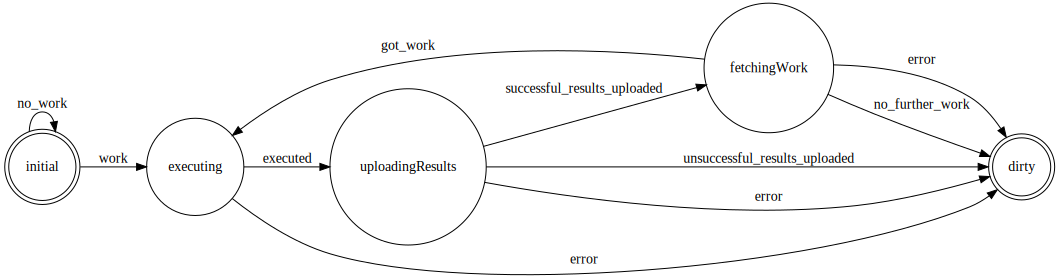
\includegraphics[width=1.0\linewidth]{../img/client_fsm}
	\caption{Client FSM}
	\label{fig:fsm}
\end{sidewaysfigure}
A finite state machine, as seen in \autoref{fig:fsm}, is used to model the client:
In the initial state the client asks periodically for work.
The client stays in the initial state if no work is available.
Otherwise it goes into execution state and tries to execute the given commands.
The client goes into an upload state after completing the execution.
After successfully uploading the images and results the client goes into the work fetching state or the dirty state depending on whether the test was successful.
A failed tests leaves the program in an undefined state.
The dirty state therefore initiates a reset.

An dirty state is also entered when an internal error happens inside the client.
In the future the client can be configured to automatically reset or leave the system unchanged for inspection.

For the implementation Akka~\cite{Akka}, AkkaFSM~\cite{AkkaFSM}, SikuliX and the Play framework~\cite{Play} are used.
They all are part of the \emph{Typesafe Reactive Platform}~\cite{TypesafeRP}.
Scalaxb~\cite{scalaxb} was used to create Scala case classes and a parser based on the test specification's XML schema.

The proof of concept does not support sequences and does not ask for additional work.
Not all operations are implemented.

The finite state machine is running as a AkkaFSM which has child actors for fetching work, uploading results and executing the test.
The error handling of Akka actors was not implemented.
Akka actors also have the drawback of not being type safe.
There is the Akky~Typed~\cite{AkkaTyped} project but it is still experimental.

\subsection{Server}

Initially the server only provides an API.
This API will be augmented by a web interface in the future.

The initial API is drafted in Swagger~\cite{Swagger} which is the basis for the \emph{Open API Initiative}~\cite{OpenAPI}.
Keeping the API completely RESTful was not a concern.
The structure may also be changed in the future to follow the \emph{JSON API}~\cite{JSONAPI} specification.

API~Studio~\cite{ApiStudio} was used for live editing and preview of the documentation.
An excerpt of the generated documentation can be seen in \autoref{fig:apiStudio}

\begin{figure*}[htbp]
	\centering
	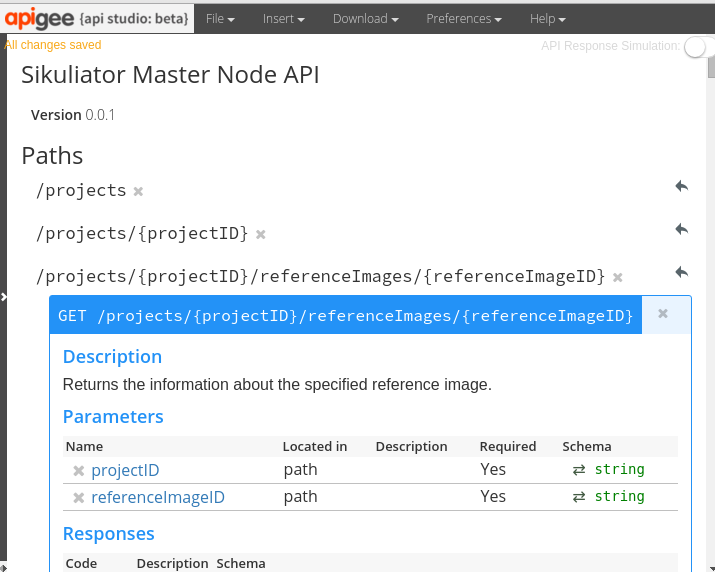
\includegraphics[width=1.0\linewidth]{../img/apiStudio}
	\caption{API Documentation excerpt generated by API~Studio}
	\label{fig:apiStudio}
\end{figure*}

The API mainly consists of a project collection.
Each project has a collection for reference images, tests and similar entities.
Some entities like tests are themselves collection of versions.

At this point only the creation of entities and getting information is possible.
Modification and deletion are not part of this proof of concept.
There are some additional differences between the API draft and the implemented API.
The implementation currently returns IDs as numbers and not as strings.
Also some operation like copying a flavour are missing even from the specification.
These will be developed based on the GUI's need.
The notification for flavours about new versions was also left out.

Only minimal validation is done.
Test and sequence specifications are not checked.

To keep the code bases consistent, Akka and the Play framework are used for the implementation.
Slick~\cite{Slick} is used for database access.

\subsection{Database}
\VMC{} uses PostgreSQL~\cite{PostgreSQL}.
Due to the familiarity, it will be used for \Sik{}, too.
Compatibility to other systems like MariaDB~\cite{MariaDB} was not regarded in this release.

The schema is based on the API draft.
The Slick definitions for the tables were generated by slick-codegen.
PostgreSQL's array type would require manual mapping to JDBC types.
The documentation on this is sparse and therefore the planned tagging feature for tests and other objects is not introduced in the proof of concept.


\section{Results}

\autoref{lst:EditorXML} shows a simple test which opens the start menu, searches for the editor, opens it and verifies that it started. 
The matching Sikuliator output is shown in \autoref{lst:EditorOutput}.
Both files are bundled with SikuliX' debug log and the used images in the documentation.
\begin{figure}
%\begin{minipage}{\linewidth}
	\begin{lstlisting}[language=XML,caption={Example test case specification},label={lst:EditorXML}]
	<?xml version="1.0" encoding="utf-8"?>
	<spec:test name="OpenEditor"  xmlns:spec="http://www.example.org/Sikuliator">
	<spec:click similarity="0.95">WindowsStartButton</spec:click>
	<spec:enterText>
	<spec:text>Editor</spec:text>
	</spec:enterText>
	<spec:click similarity="0.95">EditorButton</spec:click>
	<spec:waitForSomethingToBeThere similarity="0.95" secondsToWait="10">EditorTop</spec:waitForSomethingToBeThere>
	</spec:test>
	\end{lstlisting}
%\end{minipage}
\end{figure}

\begin{figure}
%\begin{minipage}{\linewidth}
\begin{lstlisting}[caption={Sikuliator's output for the example test case},label={lst:EditorOutput}]
clicked on WindowsStartButton
entering text: Editor
clicked on EditorButton
found EditorTop
finished successfully
\end{lstlisting}
%\end{minipage}
\end{figure}
This proof of concept shows the feasibility of the concept but is also inefficient due to no snapshot support.
It also shows the problems of engineering systems consisting of many parts and frameworks.

Picking up a new framework takes time and good documentation would help.
Integrating Play with Slick as a database layer is described in the Play documentation but some crucial parts are left out.
The necessary information is spread across different pages.
Configuring Slick differs from the default Play configurations which for example meant searching for two hours to find out that Slick needs an additional \enquote{\#} at the end of the driver class name.

Interestingly enough, error handling in Slick is hidden deep inside the documentation.
Simply enclosing a Slick query with \texttt{try} and \texttt{catch} does not work.
Therefore some initial parts of the master crash on database errors due to no error handling.
Later parts already use the \texttt{asTry} mechanism.

Some things were simply left out because it would have required too much time digging through documentations and Stackoverflow. An example is the clients's actor system shutdown because Play's dependency injection and Akka actors do not work together out of the box.

Another problem was the use of different build systems across the dependencies.
\Sik{} uses SBT~\cite{SBT} which is the common Scala build system.
SikuliX uses Maven.
The POM files use profiles to differentiate between Linux, Mac and Windows.
SBT does not support profiles.
Therefore the SikuliX libraries had to be manually downloaded and added to the project's classpath.

Writing idiomatic Scala and using the libraries' and frameworks' best practices takes experience.
The type \texttt{Option} which can be \texttt{Some(wrappedValue)} or \texttt{None} is used in large parts of the master.
Using \texttt{Try} which can be \texttt{Success(wrappedValue)} or \texttt{Failure(exception)} would be semantically better as the return type for functions which may fail like for example querying the database.
Static analysers may also help to increase code quality.

Several days were spent on researching object storage systems.
None of them are included in this small proof of concept.
But the time is not lost, for the database will not handle a lot of large binaries so
an object storage system will be introduced in a future iteration.

Deployment was not a concern so far and therefore no time was spent on creating a production build and packaging.
These two steps will again require going through the documentation.



\section{Future Roadmap}

\subsection*{GUI}
The system without a GUI is basically useless.
For the web interface there are two main contenders: Angular~2~\cite{Angular2} or Scala.js~\cite{ScalaJs}.
Scala.js would keep the whole system in one language and give type safety but requires a fully custom write of the GUI.
Angular is a common framework for single page application.
Foundation~\cite{Foundation} would probably be used as the CSS and HTML framework 
because it is one of the major frameworks and it handles things like accessibility and responsive design.

\subsection*{API}
The API will probably change when the common requests are more clear.
This should be the case when the GUI is being developed.
Also the notion of users and roles will be integrated.
This will also require authentication and authorization.

\subsection*{Testing and Static Analysis}
Testing based on Travis~\cite{Travis} will be set up and static analysers like Scalastyle~\cite{Scalastyle} or Scapegoat~\cite{Scapegoat} may be used.
Travis can set up a test database which allows running tests against a complete master node instead of mocks.
This set up will be configured while developing the API.
The only thing that Travis cannot test is the client.

\subsection*{Jenkins Integration}
Jenkins is used to build \VMC{}.
Integrating \Sik{} as the last testing step makes sense once the system is in a usable state for the average tester.

\subsection*{Documentation}
The system has to be documented for the administrator and for the end user.
Currently the system is in state of probable frequent change.
The documentation will be started while creating the GUI. 
Only the design documents like the API spec or the clients finite state machine are available until then.
Inconsistent or lacking documentation of used software was a problem while developing \Sik{}.
\Sik{} users should be spared from this frustration.

\subsection*{DSL}
The DSL will be developed at a later point in time after creating the GUI and it will introduce region support and snapshots.
The language development should be guided by the experiences made while writing several test specifications in the XML format.
This will require a large corpus to get a got feeling for common constructs and needed additions.

\subsection*{Integration of other Systems}
An object storage system will be introduced in the long term.
When the system provider is being developed it may also make sense to use available software for service discovery and health checking.
Existing identity providers may also be integrated.

%%%%%%%%%%%%%%%%%%%%%%%%%%%%%%%%%%%%

\printbibliography[notkeyword=software,resetnumbers=true,prefixnumbers=R]
\printbibliography[keyword=used,title={Used software},resetnumbers=true,prefixnumbers=US]
\printbibliography[notkeyword=used,keyword=software,title={Other software},resetnumbers=true,prefixnumbers=OS]

\end{document}


